\chapter{Smart Contract and Distributed Ledger Technology}

\section{Introduction}
With the arrival of Blockchain technology as a form of Distributed Ledger Technology, the rule of bitcoin in this field is on increase.  Block chain enables developer to create diverse distributed application. One of the novel approach in this field is Ethereum platform which is the turing-compelete system used in smart contract.\\
Smart contract is the part of code in block chain without ....TODO.
Block chain is the chain of block (participant computer) over network and provides a truth worthy mechanism to facilitate distributed contract in secure way.\\
TODO
\\
In this paper, we attempt to investigate if Link data in the combination with blockchain to realize the distributed semantic web application.
 TODO 
 \section{Ledger}
 \subsection{Destributed Vs. Undestributed }
 
 \section{Distributed Ledger Technology}
 Is the method of keeping distributed ledger on networks of computer. DLT use consensus technique for adding new node(participant) over network. Similarly, This is the digital record that shared across participant and the records hold by each node or participant. The term 'block chain' is a most well-known type of DLT and are used by many best-known instances of DLT.\\
 It goes without saying that distributed ledger can be either permission less or with permission, regarding to be private or public. 
 Most of the distrubuted ledger is permission less and public means any one can easily join to network and see all entries. But in financial fields, distributed ledgers are restricted to membership of each participant and they are 'commissioned ' and 'private' network. Furthermore, in financial fields exist also commercial sensitivity about the privacy of data related to each participant. In the other word, no one wants that data to be seen by the other participant. therefore, participants are able to see their own data and transaction on the network [44].\\
 recently, blockchain as a type of distributed ledger become most popular and widely used in diverse fields. ledgers such as Ethereum extends initial bitcoin blockchain with features such as smart contracts that enable to distribute data on blockchain in secure way.
 In addition, there is incrementally need to integrate data stored in distributed ledger with other external sources. And also integrate smart contract with the service available on the web. This is where linke-data comes to play to provide sufficient access to data and smart contract also stored on Ehereum blockchain via semantic web technology stack.[p1431] 
 
\section{smart contract}
Smart contract in computer science is the piece of code which is designed to execute certain terms if the predefined conditions are met. These terms are embedded and preformed on distributed ledger. As a compared to traditional contract that includes third party to execute terms of condition , smart contract has low transaction fees and is more profitable. Conception of smart contract is defined in distinct schools or terms: Smart legal contract that consider contract's legitimacy and includes right and obligations of different parties which are legally applicable. Second school focus on the main code of smart contract run successfully and required legal smart contract. One definition that performs this job well is that of Clack, Bakshi and Braine [] that is comprehensive meaning that covers both smart legal contract and smart contract code:\\
\textit{A smart contract is an automatable and enforceable agreement. Automatable by computer, although some parts may require human input and control. Enforceable either by legal enforcement of rights and obligations or via tamper-proof execution of computer code.}[]
Sometimes, smart contract and DLT are remembered as same thing, but actually not. They are different technologies which are complementary of each other. However, there are several platforms in DLT on which smart contract can execute. By existing computer and capability of execurting code, why have not smart contracts developed?\\
This question indicates the highlighted role of smart contract and DLT and the relationship between each other.
It is true that computer is capable of executing an event such as payment of a contact upon satisfaction of pre-defined conditions. But, that would have meant that both partied requires to have programmed on own computer. subsequently,they need different instance to run on their computers and the version of their code and program may differ that would be other issue. 
What DLT has done, is that creating unique versties a to bind to parties to each other by embedded code in distributed ledger. More importantly, DLT ensure both parties to have secure transaction and contract will executed automatically without any possibility of tampering from other sides. This is the accurate description of smart contract as 'self-executed' and 'self-enforced'. 
With the advent of distributed ledger, needing for efficient query of diverse data  and indexing entries become more important.  [44]   \\
Within the blockchain, Smart contract is actually code inside the block and it triggers by receiving a transaction or massage and send the transactioninrespose of transaction that has received then it can read, write or create contract. \\
smart contract is the independent factor an be half of user to preform some operations the as long to users goals. These goals are programmed inside the contracts as code. Each contact controlled own Ether, key as long lasting storage to follow the constant variables.[29]\\
Let us clarify more by one example:
Consider blockchain network  where Bob, Alice and Carol are participant and there exist 2 assets X and Y. Box use the smart contract that defines three functions: \textit{'deposit'}: store unit of X into contract, \textit{'trade'} send back one unit if X instead of  five unit of Y  and \textit{'withdraw'} to roll back all asset into the contract.
Bob start activating smart contract by calling the \textit{'deposit'} function and moving 3 unit of X asset into contract and record it in the blockchain. Alice has 12 unit of Y, and sending transaction and 'trade' 10 unit of Y and get back 2 unit of Y and recorded into blockchain as well. Bob signed transaction to \textit{'withdraw'} function. Contract check signiture and \textit{'withdraw'} is called by owner, then transfer all deposits 1 unit of x and 10 unit of Y to Bob. [14]\\
Let us extract the features of smart contact out of this example:

 \textbf{-} Contract has its own states and controll over own assets.\\
 \textbf{-} Contract allows us to do bussiness logic in code. \\
 \textbf{-} Contract is deterministic means for the same input produce same output.\\
 \textbf{-} Correct smart contract describes all possible outcome.\\
 \textbf{-} Relationship between participants are explained by data.\\
 \textbf{-} Smart contract is triggered by receiving transaction and sent transaction afterwards.\\
 \textbf{-} Since contract stores on blockchain, that can be visible by every participcant on network.\\
 \textbf{-} Each participant can get cryptographically verifiable trace of contract operation due to \textit{sign} message.\\

Smart contracts have state, which can be updated by a contract when it is executed. The blockchain keeps a record of all previous states of a contract beacause overwrittng previous state would involve overwriting records earlier in the blockchain. Smart contracts can be used to implement dynamic data storage with history in the Ethereum environment.[Ethgrap]
   





\subsection{Validation of Smart contract38}

\subsection{Semantic of Smart contract34}

Whereas Computer programmer deal with validation of contract, Then the semantic aspect of contract is considerable case in this field and thus the \textit{meaning} of contract should not be ambiguous.Legal contract has 2 main aspect:
 \begin{enumerate}
 	
 	 \item \textbf{Operational aspect}[44]
 	 \item \textbf{Non-operational aspect} [44]
 	
 \end{enumerate}

\subsection{Different models of smart contracts}[44]
There are two models of smart legal contract. However, most implementation of smart contract is near to the term operational clause, rather then non-operational clause.
\begin{enumerate}
	\item external contract
	\item Internal contract
\end{enumerate}
\subsection{Semantic Analysis38}


\section{Block chain}
Blockchains are the distributed records for digital events and they are structured as chain of linked data stored in individual database or computer over network.[p1431]
Block chain are organized into blocks. Each  block is identified by cryptography hash that refers to hash of previous block. this create links between block. Thus, it create the chain of blocks wherein Blocks are held the copy of blockchain structure. The initial block created manually, is known as \textit {genesis block} and the other node will add to block chain after a process of consensus between nodes. The distributed consensus method which allow to add new block or item into blockchain that is verified as legitimate. This process would be done by some computational work called as Proof Of Work (POW) or mining.
All blocks in blockchain hold small amount of data which need to be secure before distributing over all participating computer over network and are visible by having public key for all participant but not modifiable. These data time stamped and provide the time of adding that block.)

 \begin{center}
 	\begin{figure}[htb!]
 		
 		\begin{minipage}{0.55\linewidth}
 			\centering
 			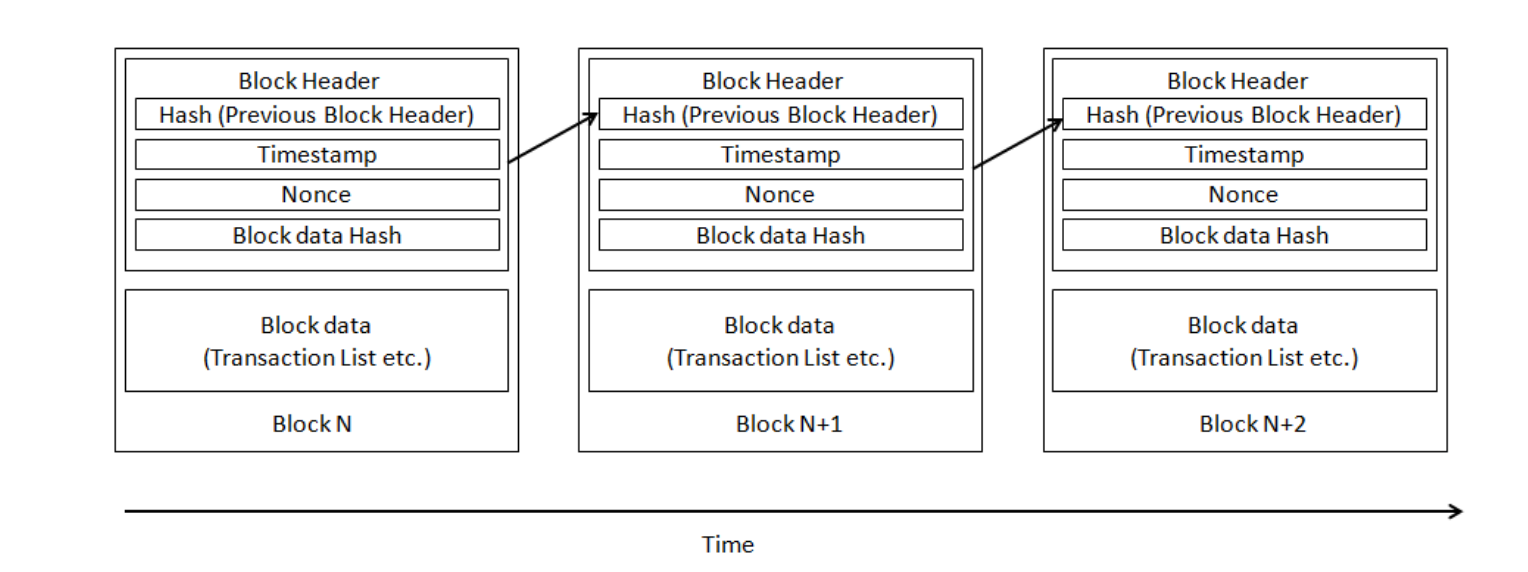
\includegraphics[width=1.95\textwidth]{images/chap01_BlockChain.png}
 		\end{minipage}
 		\caption[Generic chain og blocks]{[18740]}
 		
 		
 	\end{figure}
 	
 \end{center}
Blockchain has four main concept: \textit{P2P network:} node can interact with each other using private for sign transaction and public keys sre used as address that can be reachable on te network. \\
   \textit{Open distributed ledge}: It is like book containg all transactions that each node has the copy of data and there is no centrellized entity and any one can see assets and how much assets has each node.Therefor, they can decide about the validity of transactions.\\
   \textit{Schronization}: As, all node have one copy of ledger. Therefor, sycronization should prefome overall networks and by adddning new item or one new transaction should be performe in public and consensus needed to valid this transaction.\\
   \textit{Mining: }In the distributed ledger, all nodes can not receive transaction simultaneously. For adding new item in the blockchain, consensus of all nodes are needed. Thus there is need to prevent every onn node to add transaction into blockchain. Miners are the unique nodes that can add transaction to that chain. Miners attempts to validate the first transaction to add into chain.  
There are several distributed system based on consensus, but the one outstanding feature that makes blockchain  more prominent then the others is that :
 Only single record stores in each participant computer. This provides transparency of transaction. Whilst storing whole 
records over all networks of participating computer mitigate the probability of losing infrastructure.[2016 book 491]\\
And blockchain is the sole technology which fulfill such properties:\textit{(a)trustless}: There is no need to verify involved identities in transaction. \textit{(ii) Permissionless}: there is neither permission nor controlling for participants in network.   \textit{(iii)censorship resistant}: Anyone can trades on blockchain and just cryptographic algorithm governs the operation that entities(participants) can trust it.[50]


this feature and above reason make the block chain as powerful and most secure technology in commercial events over network.[50]

\begin{center}
	\begin{figure}[htb!]
		
		\begin{minipage}{0.55\linewidth}
			\centering
			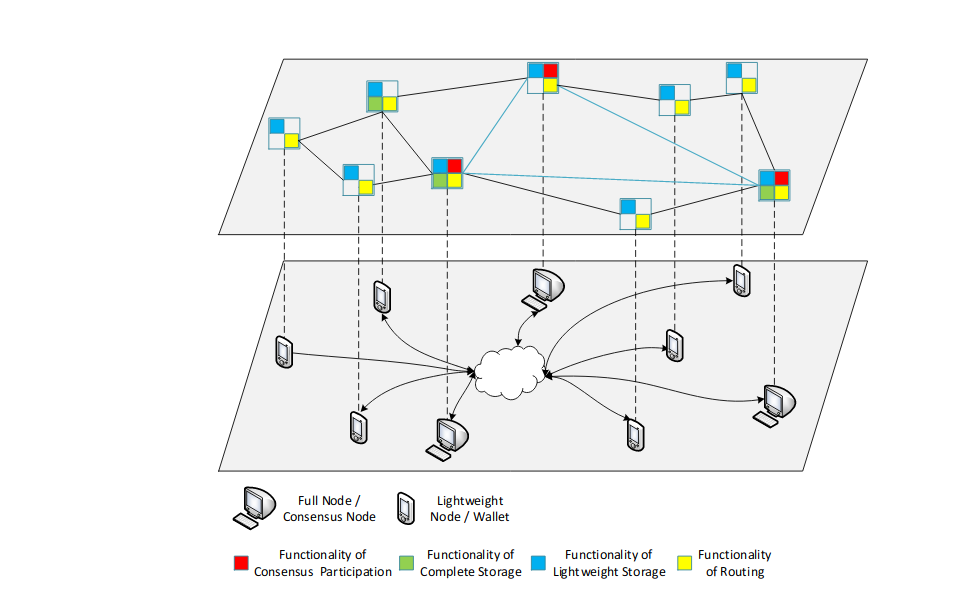
\includegraphics[width=1.95\textwidth]{images/chap01_P2P.png}
		\end{minipage}
		\caption[Permissionless blockchain network. The P2P links between consensus nodes are shown in blue.]{[60]}
		
		
	\end{figure}
	
\end{center}

\textbf{Permissionless / public Blockchain} This blockchain allows any0ne to join to network and create consensus such Bitcoin nd Ethereum. oin permissionless  blockchain any miner can create consensus mechnism such as proof of work, proof of stack to validate transaction. but as this mechanism is decentraliised the rate of validity of function and scalabilitiy is low.[30]

\textbf{Permissioned/ Private Blockchain}: this blockchain, only restricted  participant has right to validate transaction. Threfore, it provides better privacy and scalability. Unlike permissionless blockchain, this blockchain does not have  mining computation to reach the consenus because all participant are known in this network. [30]
\textbf{Privare Key/wallet}

\subsection{Bitcoin} 
The basic goal of blockchain technolgy is to ensure people form truthworthy and ligimacy of transactions. Blockchain initially used to enhance commercial transaction through currency called Bitcoin. \\
Bitcoin is the digital records or cryptocurrency that is accept by users involved in transaction. in fact, Bitcoin is the financial use cases of this powefull technology.[50]
Bitcoin is the list of blocks of transactions. Each block in blockchain is identifeid by hash algorithm on the top of the block.
Bitcoin is introduced by consensus mechanism of blockchain, it is well known implimentation of decentralized cryptocurrency.\\
Bitcoin is the limit of block, wherein each block is verified by hash algorithm using SHA256 cryptgraphic on the top of block. Each block encompass the hash of its parent (previous block) in the own header that refuse to it.
It forms block list wherein each block refers to previous block in the list name  genesis block[1]. Altering in block implies to create new blockon the top. Since, each block contains the hash of its parent creating new block is expensive and  needs proof of work that the miners allow the add new block.[1]

\subsection{Proof Of Work}
Is consensus algorithm in blockchain without any central algorithm that used to confirm transaction and add new block. With POW miners compete to complete its own transaction first into blockchain and get rewards(e.g: Bitcoin, Ether, ...).\\
Miners connected to blockchain and accomplish task validating transaction to add new block bc solving cryptographic puzzle[1].
TODO
\subsection{Mining}
Is an process if computation on the blockchain in order to verify and add block.[29]
TODO

\subsection{Merkler Tree}
all transactions are stored in tree structure wherein leafs contain transactions and internal node contain the hash of its sub tree and single root also contains the hash of two children  and represent top of tree. The purpose of bottom up hashing is that, if attacker attempts to create fake transaction into bottom of tree. This will change the node above and subsequently change the root. Thus altering the hash of block causing to register new block. Only the sequence of hash form root the leaf called the Merkler tree. [8a]   
\begin{center}
	\begin{figure}[htb!]
		
		\begin{minipage}{0.55\linewidth}
			\centering
			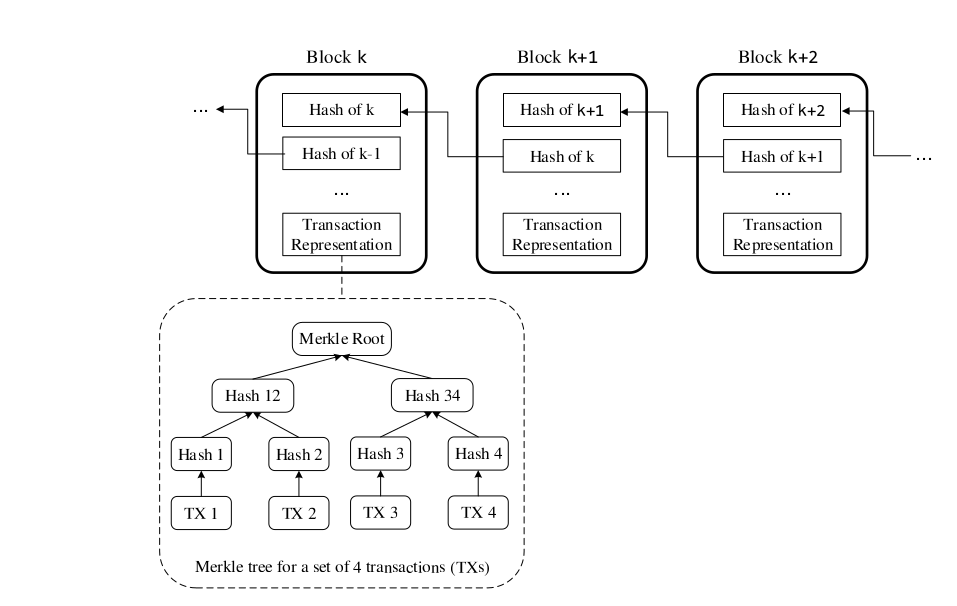
\includegraphics[width=1.85\textwidth]{images/chap01_Markler_tree.png}
		\end{minipage}
		\caption{Illustration of chain of blocks and  markler tree in single block}{[60]}
		
		
	\end{figure}
	
\end{center}

\subsection{Hash Function}
It is mathematicaly method to applay cyptografic(secret writting) function. hash function is deterministic means for an input produce same output each time. altering data generate the different output. 
According to Wikipedia, the security level of hash function has different properties: \\
\begin{itemize}
	
	\item {Pre-image resistance}: It s not easy, for initial input with /{h /}  hash value find the output value \{m\} , in a way that \{h = hash(m) \}
	
	\item {Second pre-image resistance}: it is not easy, for input \(m_1\)  find another input \(m_2\)   in way that \()hash(m_1)  = hash(m_2)\) and both have same result.
	\item {Collisio Resistance} : it is difficult to find two different input \(m_1  , m_2)\) that have same output in way that\( hash(m_1) = hash(m_2)\).\\
\end{itemize}
	Hash function used in blockchain and it is the most secure hashing algorithm is SHA256 which that provide the combination for an given input with 256 bit length. Using SHA 256 in blockchain makes to be impossible to dublicate hash because there are diverse combination of this input with this length and it requires huge amout of computaional works. That means thare are \( 2^ {256} \) hash values.
	
     \begin{center}
     	\begin{tabular}{c | c }
     	
     	 Input value  & SHA 256, message hash\\ 
     	 
        \hline
          1   &  6b86b273ff34fce19d6b804eff5a3f5747ada4eaa22f1d49c01e52ddb7875b4b \\
        \hline
     	  2    &   d4735e3a265e16eee03f59718b9b5d03019c07d8b6c51f90da3a666eec13ab35	\\
     	 \hline
     	 Blockchain & 625da44e4eaf58d61cf048d168aa6f5e492dea166d8bb54ec06c30de07db57e1 \\	
        \end{tabular}
        
     \end{center}


\subsection{Header} contains timetamp, nonce, previous hash, ...
\subsection{Nonce} it stands for \textit{number ued only once}. It is intger number and along with block data, number and previous hash use as input in SHA256 function to generate current block hash. We used this nonce to vary the hash of current block and without modifying  the data inside the block.the By the usage of nonce, miner can generate valid hash, adding first  own block into blockchain and get the reward.


\subsection{Transaction} transfer data (asset) between users, an transaction contains inforamtion such:\
- The recipents which message to send.
- Signiture of sender 
- A mount of ether to transfer
-Structure value, the maximum number of computational step that transaction is allowed to do 
- Gaspreice, fees that should pay.[29]

\subsection{Proof Of Stack} 

\subsection{Cryptographic hash functionn}
\section{Ethereumt}
Ethereum is the decentralized virtual machine based on block chain. Ethereum block chain stores codes of program and transaction data both on both on block chain. The code of contract is fed into block chain without address. Afterwards, the contract which already added to block chain and assigned address. As said before,the code of contract is unmodified, unlike contract's state that could be altered any time.
In Ethereum virtual machine, node or block besides adding the transaction to ledger, render contract codes and control the state in virtual machine.\\

TODO
Undoing smart contract etheruem ??
attack on ethereum smart contract.
\subsection{Security in Smart contract}

An  analysis  of  existing  smart  contracts  by  Bartoletti  andPompianu[7]shows that the Bitcoin and Ethereum platformmainly  focus  on  financial  contracts.  In  other  words,  mostsmart contract program code defines how assets (money) move.Therefore,  it  is  crucial  that  contract  execution  is  performedcorrectly.  The  direct  handling  of  assets  means  that  flawsare  more  likely  to  be  security  relevant  and  have  greaterdirect financial consequences than bugs in typical applications.Incidents, like the value overflow incident in Bitcoin [8], or theDAO hack [9] in Ethereum, caused a hard fork of the blockchain
to  nullify  the  malicious  transactions.  These  incidents  showthat  security  issues  have  been  used  for  fraudulent  purposesruthlessly in the past. A survey of possible attacks on Ethereumcontracts  was  published  by  Atzei  et  al.[10]and  lists  12vulnerabilities that are assigned by context to Solidity, the EVM,and blockchain peculiarities itself. Many of these vulnerabilitiescan be addressed by following best practices for writing securesmart contracts, which are scattered throughout the Ethereumcommunity [11,12] and different Ethereum blogs. Most bestpractices mainly contain information about typical pitfalls toavoid and the description of favourable design and problemapproaches. The latter being the focus of this paper in orderto collate smart contract security design patterns.[scsecurity]
\subsection{Vulnerabilities in Ethereum Smart Contracts}

Author in this section categorized the vulnerabilities in smart contracts into three classes(solidity, Ethereum virtual machine, blockchain):\\
\begin{center}
   \begin{tabular}{c |c }
   	\hline
   	    cal1 & cal2 \\
   	\hline
   	  \multirow{2}{4em}{Solidity} & Call to the unknown \\ & Gasless send \\ & Exception disorders  \\ & Type casts \\ & Reentrancy \\ & Keeping secrets \\
   	\hline 
   	  \multirow{2}{4em}{EVM}& Immutable bugs \\ & Ether lost in trasfer \\ & Stack size limit \\
   	\hline  
   	 \multirow{2}{4em}{Blockchain} & Unpredictable state \\ & Generating randomness \\ & Time constraints \\
   	\hline
   \end{tabular}	 
 
\end{center}
\textbf{- Call to Unknown:} One invokes the function and transfer the ether to the counterpart. If there is no signature in the given address, then the fallback function is executed.\\ 
for example: In the contract \textit{Alice} and  \textit{Bob}:\\
 Alice has \textbf
{Ping} function and Bob invokes the Alice contract (\textbf{ping} function) via direct call. If there is any mistype in calling function such as \textit{int} instead of \textit{Uint} call to the \textbf{ping} return fallback function. \\

\texttt{\color{red}contract \color{black}Alice \{ \color{red}function \color{black}ping (\color{red} uint \color{black}) \color{red}returns \color{black}( \color{red}uint \color{black}) ; \} }\\
\texttt{\color{red}contract \color{black}Bob
	\{ \color{red}function \color{black}pong (Alice c) \{c.ping (42); \} \}}
\\
Or in another contract: \\
\texttt{c.\color{red}call . value \color{black}(amount)(bytes4(sha3("ping(uint256)")),n); }\\
function \textbf{ping} in contract \textbf{c}: called function is identified by hash signature.\\
\textbf{amount } is the much of \textit{wei} that is to transfer to contarct \textbf{c}.\\
\textbf{n}  is parameter in \textbf{ c}. If the function with this signature does not exist in the contract the fallback function is executed.  
\\

\textbf{- Exception disorder: } this is occurred in situation such as: executation run out of gas, call stack reaches to its limit and \textit{throw} commend is executed.
For instance in this contract:\\
\texttt{\color{red}contract \color{black}Alice \{ \color{red}function \color{black}ping (\color{red} uint \color{black}) \color{red}returns \color{black}( \color{red}uint \color{black}) ; \}}\\
 \texttt{ \color{red}contract \color{black}Bob
 	\{\color{red} uint \color{black} x=0;
 	\\ \color{red}function \color{black}pong ( Alice c ) \{ x= 1; c.ping (42); x=2; \} \}}\\
 
 There are two possibility of \textit{call }function: 
 \begin{itemize}[label={},leftmargin=12.5mm]
  \item User invokes Bob function, therefore, \textbf{ping} throw exeption and execution stops. Side effect of all transactions are reverted and \(x=0\) after transaction.
  \item  Bob invokes \textbf{Ping } via call, Only side effect of invocation reverted, call returns fail, execution continue and \(x=2\)  after transaction.
 \end{itemize}
\textbf{Gasless send: }\textbf{send} function , transfer ether to contract. This function compiled the same way of \textit{call }function without signature and returns \textit{out of gas} exception.\\
Assume \textit{call} has no signature, so it invokes \textit{callee's } fallbac  function. However  the upper bound of unit of gas is 2300 that is avaiable to \textit{callee } and is executable.

\begin{multicols}{2}
	\texttt{
		\color{black} 1 -\color{red}contract \color{black}C \{\\
		\color{red}function \color{black}pay(\color{red}uint \color{black}n, \color{red}address \color{black}d) \{\\
		d.send(n) ;\\
		    \hspace*{4mm}\}\\
		\}}
	
	 
	\columnbreak
	
	
	\texttt{\color{black} 2 - \color{red}contract \color{black}D1 \{\\
			\color{red}uint public \color{black}count = 0;\\
			\color{red}function \color{black}() \{ count ++; \}\\
	       \}
		\color{red}contract \color{black}D2 \{ \color{red}function \color{black}() \{\} \}}
	 
\end{multicols}

\textbf{Type casts}
\textbf{Reentrancy}
\textbf{Keeping secrets}
\textbf{Immutable bugs}
\textbf{Ether lost in transfer}
\textbf{Stack size limit}
\textbf{Unpredictable state}
\textbf{Generating randomness}
\textbf{Time constraints}
